{\bf Problem 4: Answers}

\begin{enumerate}
    \item[] a., b., c.
\end{enumerate}

\begin{quote}
    We see that a deep network performs significantly better than a wide network with the same number of parameters.
    The deep network reaches comparable levels of performance to the wide in one epoch compared to eighteen epochs. 
    This performance is shown in the following tables and plotted in figures 3 and 4.
    The reason for the deep network's better performance is likely due to there being more nonlinearities in the deeper model so the data are more immediately fit.

    \begin{center}
	\begin{tabular}{ |c|c|c|c|c| } 
	    \multicolumn{5}{c}{Model Performance} \\	
	    \hline
	    & \multicolumn{2}{c|}{Wide Net} & \multicolumn{2}{c|}{Deep Net} \\
	    \hline
	    & Training & Testing & Training & Testing \\
	    \hline
	    Accuracy & 0.9904 & 0.9749 & 0.9911 & 0.9718 \\ 
	    \hline
	    Loss & 0.0336 & 0.0844 & 0.0320 & 0.0928 \\ 
	    \hline
	\end{tabular}
	\begin{tabular}{ |c|c|c|c|c| } 
	    \multicolumn{5}{c}{Model Details} \\
	    \hline	
	    & \multicolumn{2}{c|}{Wide Net} & \multicolumn{2}{c|}{Deep Net} \\
	    \hline
	    Number of Parameters & \multicolumn{2}{c|}{50890} & \multicolumn{2}{c|}{50890} \\
	    \hline
	    Epochs trained & \multicolumn{2}{c|}{18} & \multicolumn{2}{c|}{1} \\
	    \hline
	\end{tabular}
    \end{center}

    \begin{figure}[h!]
	\centering
	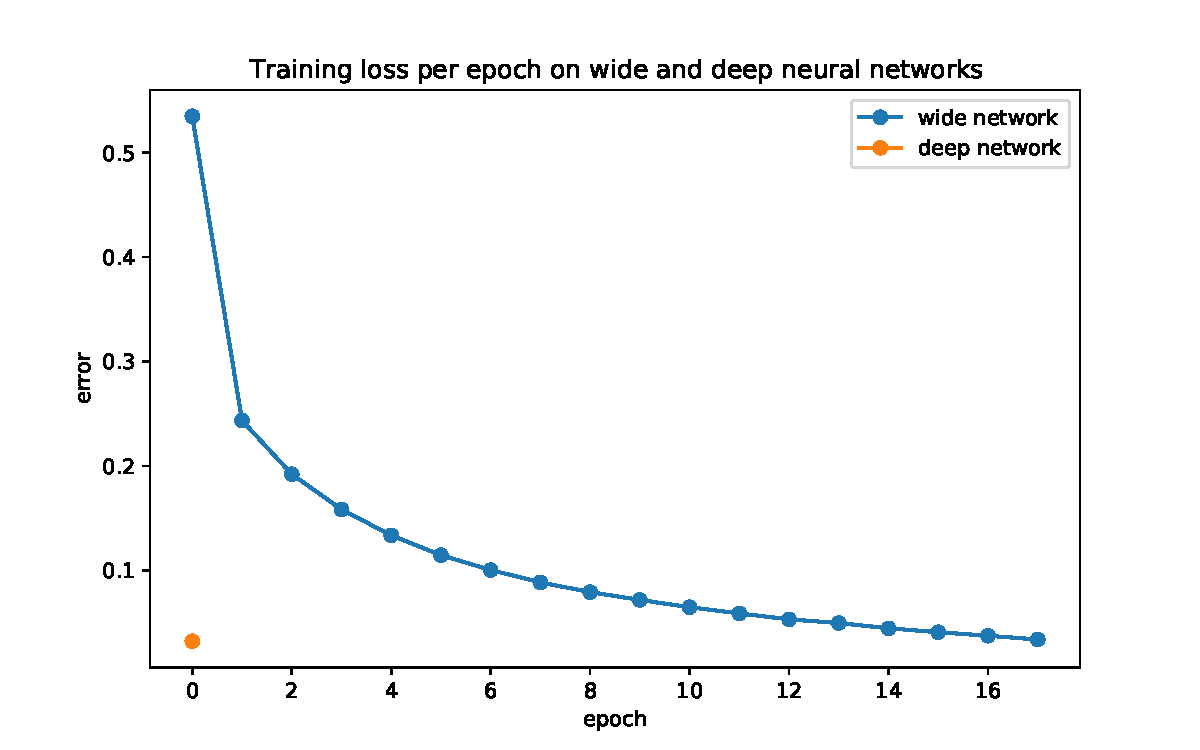
\includegraphics[width=0.8\linewidth]{../plots/4_losses.pdf}
	\caption{}
    \end{figure}
    \begin{figure}[h!]
	\centering
	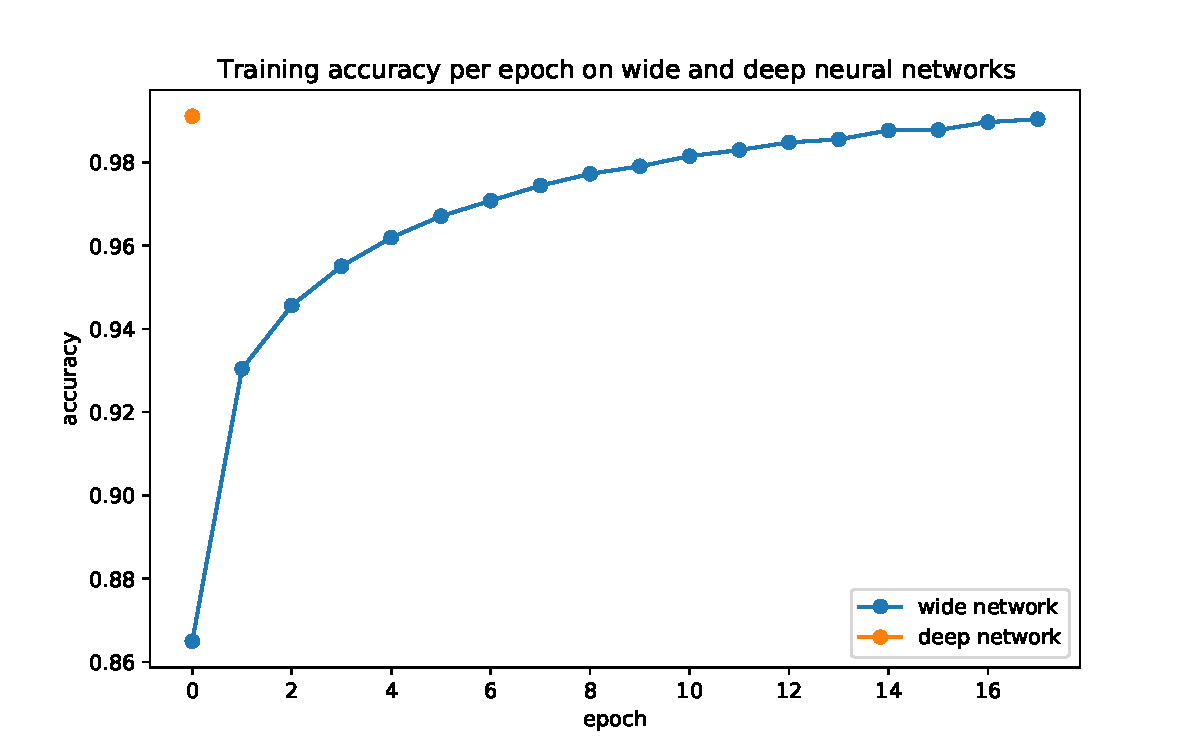
\includegraphics[width=0.8\linewidth]{../plots/4_accuracies.pdf}
	\caption{}
    \end{figure}

{\bf Problem 4: Code}
\lstinputlisting[language=Python]{../code/p4.py}

\end{quote}
